\documentclass[a4paper,11pt,oneside]{memoir}

% Castellano
\usepackage[spanish,es-tabla]{babel}
\selectlanguage{spanish}
\usepackage[utf8]{inputenc}
\usepackage{placeins}

\RequirePackage{booktabs}
\RequirePackage[table]{xcolor}
\RequirePackage{xtab}
\RequirePackage{multirow}

% Links
\usepackage[colorlinks]{hyperref}
\hypersetup{
	allcolors = {red}
}

% Ecuaciones
\usepackage{amsmath}

% Rutas de fichero / paquete
\newcommand{\ruta}[1]{{\sffamily #1}}

% Párrafos
\nonzeroparskip


% Imagenes
\usepackage{graphicx}
\newcommand{\imagen}[2]{
	\begin{figure}[!h]
		\centering
		\includegraphics[width=0.9\textwidth]{#1}
		\caption{#2}\label{fig:#1}
	\end{figure}
	\FloatBarrier
}

\newcommand{\imagenflotante}[2]{
	\begin{figure}%[!h]
		\centering
		\includegraphics[width=0.9\textwidth]{#1}
		\caption{#2}\label{fig:#1}
	\end{figure}
}



% El comando \figura nos permite insertar figuras comodamente, y utilizando
% siempre el mismo formato. Los parametros son:
% 1 -> Porcentaje del ancho de página que ocupará la figura (de 0 a 1)
% 2 --> Fichero de la imagen
% 3 --> Texto a pie de imagen
% 4 --> Etiqueta (label) para referencias
% 5 --> Opciones que queramos pasarle al \includegraphics
% 6 --> Opciones de posicionamiento a pasarle a \begin{figure}
\newcommand{\figuraConPosicion}[6]{%
  \setlength{\anchoFloat}{#1\textwidth}%
  \addtolength{\anchoFloat}{-4\fboxsep}%
  \setlength{\anchoFigura}{\anchoFloat}%
  \begin{figure}[#6]
    \begin{center}%
      \Ovalbox{%
        \begin{minipage}{\anchoFloat}%
          \begin{center}%
            \includegraphics[width=\anchoFigura,#5]{#2}%
            \caption{#3}%
            \label{#4}%
          \end{center}%
        \end{minipage}
      }%
    \end{center}%
  \end{figure}%
}

%
% Comando para incluir imágenes en formato apaisado (sin marco).
\newcommand{\figuraApaisadaSinMarco}[5]{%
  \begin{figure}%
    \begin{center}%
    \includegraphics[angle=90,height=#1\textheight,#5]{#2}%
    \caption{#3}%
    \label{#4}%
    \end{center}%
  \end{figure}%
}
% Para las tablas
\newcommand{\otoprule}{\midrule [\heavyrulewidth]}
%
% Nuevo comando para tablas pequeñas (menos de una página).
\newcommand{\tablaSmall}[5]{%
 \begin{table}
  \begin{center}
   \rowcolors {2}{gray!35}{}
   \begin{tabular}{#2}
    \toprule
    #4
    \otoprule
    #5
    \bottomrule
   \end{tabular}
   \caption{#1}
   \label{tabla:#3}
  \end{center}
 \end{table}
}

%
% Nuevo comando para tablas pequeñas (menos de una página).
\newcommand{\tablaSmallSinColores}[5]{%
 \begin{table}[H]
  \begin{center}
   \begin{tabular}{#2}
    \toprule
    #4
    \otoprule
    #5
    \bottomrule
   \end{tabular}
   \caption{#1}
   \label{tabla:#3}
  \end{center}
 \end{table}
}

\newcommand{\tablaApaisadaSmall}[5]{%
\begin{landscape}
  \begin{table}
   \begin{center}
    \rowcolors {2}{gray!35}{}
    \begin{tabular}{#2}
     \toprule
     #4
     \otoprule
     #5
     \bottomrule
    \end{tabular}
    \caption{#1}
    \label{tabla:#3}
   \end{center}
  \end{table}
\end{landscape}
}

%
% Nuevo comando para tablas grandes con cabecera y filas alternas coloreadas en gris.
\newcommand{\tabla}[6]{%
  \begin{center}
    \tablefirsthead{
      \toprule
      #5
      \otoprule
    }
    \tablehead{
      \multicolumn{#3}{l}{\small\sl continúa desde la página anterior}\\
      \toprule
      #5
      \otoprule
    }
    \tabletail{
      \hline
      \multicolumn{#3}{r}{\small\sl continúa en la página siguiente}\\
    }
    \tablelasttail{
      \hline
    }
    \bottomcaption{#1}
    \rowcolors {2}{gray!35}{}
    \begin{xtabular}{#2}
      #6
      \bottomrule
    \end{xtabular}
    \label{tabla:#4}
  \end{center}
}

%
% Nuevo comando para tablas grandes con cabecera.
\newcommand{\tablaSinColores}[6]{%
  \begin{center}
    \tablefirsthead{
      \toprule
      #5
      \otoprule
    }
    \tablehead{
      \multicolumn{#3}{l}{\small\sl continúa desde la página anterior}\\
      \toprule
      #5
      \otoprule
    }
    \tabletail{
      \hline
      \multicolumn{#3}{r}{\small\sl continúa en la página siguiente}\\
    }
    \tablelasttail{
      \hline
    }
    \bottomcaption{#1}
    \begin{xtabular}{#2}
      #6
      \bottomrule
    \end{xtabular}
    \label{tabla:#4}
  \end{center}
}

%
% Nuevo comando para tablas grandes sin cabecera.
\newcommand{\tablaSinCabecera}[5]{%
  \begin{center}
    \tablefirsthead{
      \toprule
    }
    \tablehead{
      \multicolumn{#3}{l}{\small\sl continúa desde la página anterior}\\
      \hline
    }
    \tabletail{
      \hline
      \multicolumn{#3}{r}{\small\sl continúa en la página siguiente}\\
    }
    \tablelasttail{
      \hline
    }
    \bottomcaption{#1}
  \begin{xtabular}{#2}
    #5
   \bottomrule
  \end{xtabular}
  \label{tabla:#4}
  \end{center}
}



\definecolor{cgoLight}{HTML}{EEEEEE}
\definecolor{cgoExtralight}{HTML}{FFFFFF}

%
% Nuevo comando para tablas grandes sin cabecera.
\newcommand{\tablaSinCabeceraConBandas}[5]{%
  \begin{center}
    \tablefirsthead{
      \toprule
    }
    \tablehead{
      \multicolumn{#3}{l}{\small\sl continúa desde la página anterior}\\
      \hline
    }
    \tabletail{
      \hline
      \multicolumn{#3}{r}{\small\sl continúa en la página siguiente}\\
    }
    \tablelasttail{
      \hline
    }
    \bottomcaption{#1}
    \rowcolors[]{1}{cgoExtralight}{cgoLight}

  \begin{xtabular}{#2}
    #5
   \bottomrule
  \end{xtabular}
  \label{tabla:#4}
  \end{center}
}


















\graphicspath{ {./img/} }

% Capítulos
\chapterstyle{bianchi}
\newcommand{\capitulo}[2]{
	\setcounter{chapter}{#1}
	\setcounter{section}{0}
	\chapter*{#2}
	\addcontentsline{toc}{chapter}{#2}
	\markboth{#2}{#2}
}

% Apéndices
\renewcommand{\appendixname}{Apéndice}
\renewcommand*\cftappendixname{\appendixname}

\newcommand{\apendice}[1]{
	%\renewcommand{\thechapter}{A}
	\chapter{#1}
}

\renewcommand*\cftappendixname{\appendixname\ }

% Formato de portada
\makeatletter
\usepackage{xcolor}
\newcommand{\tutor}[1]{\def\@tutor{#1}}
\newcommand{\course}[1]{\def\@course{#1}}
\definecolor{cpardoBox}{HTML}{E6E6FF}
\def\maketitle{
  \null
  \thispagestyle{empty}
  % Cabecera ----------------
\noindent
\includegraphics[width=\textwidth]{cabecera}\vspace{1cm}%
  \vfill
  % Título proyecto y escudo informática ----------------
  \colorbox{cpardoBox}{%
    \begin{minipage}{.8\textwidth}
      \vspace{.5cm}\Large
      \begin{center}
      \textbf{TFG del Grado en Ingeniería Informática}\vspace{.6cm}\\
      \textbf{\LARGE\@title{}}
      \end{center}
      \vspace{.2cm}
    \end{minipage}

  }%
  \hfill\begin{minipage}{.20\textwidth}
    
\includegraphics[width=\textwidth]{escudoInfor}
  \end{minipage}
  \vfill
  % Datos de alumno, curso y tutores ------------------
  \begin{center}%
  {%
    \noindent\LARGE
    Presentado por \@author{}\\ 
    en Universidad de Burgos --- \@date{}\\
    Tutor: \@tutor{}\\
  }%
  \end{center}%
  \null
  \cleardoublepage
  }
\makeatother

\newcommand{\nombre}{Nombre del alumno} %%% cambio de comando

% Datos de portada
\title{título del TFG}
\author{\nombre}
\tutor{nombre tutor}
\date{\today}

\begin{document}

\maketitle


\newpage\null\thispagestyle{empty}\newpage


%%%%%%%%%%%%%%%%%%%%%%%%%%%%%%%%%%%%%%%%%%%%%%%%%%%%%%%%%%%%%%%%%%%%%%%%%%%%%%%%%%%%%%%%
\thispagestyle{empty}


\noindent
\includegraphics[width=\textwidth]{cabecera}\vspace{1cm}

\noindent D. nombre tutor, profesor del departamento de nombre departamento, área de nombre área.

\noindent Expone:

\noindent Que el alumno D. \nombre, con DNI dni, ha realizado el Trabajo final de Grado en Ingeniería Informática titulado título de TFG. 

\noindent Y que dicho trabajo ha sido realizado por el alumno bajo la dirección del que suscribe, en virtud de lo cual se autoriza su presentación y defensa.

\begin{center} %\large
En Burgos, {\large \today}
\end{center}

\vfill\vfill\vfill

% Author and supervisor
\begin{minipage}{0.45\textwidth}
\begin{flushleft} %\large
Vº. Bº. del Tutor:\\[2cm]
D. nombre tutor
\end{flushleft}
\end{minipage}
\hfill
\begin{minipage}{0.45\textwidth}
\begin{flushleft} %\large
Vº. Bº. del co-tutor:\\[2cm]
D. nombre co-tutor
\end{flushleft}
\end{minipage}
\hfill

\vfill

% para casos con solo un tutor comentar lo anterior
% y descomentar lo siguiente
%Vº. Bº. del Tutor:\\[2cm]
%D. nombre tutor


\newpage\null\thispagestyle{empty}\newpage




\frontmatter

% Abstract en castellano
\renewcommand*\abstractname{Resumen}
\begin{abstract}
En este primer apartado se hace una \textbf{breve} presentación del tema que se aborda en el proyecto.
\end{abstract}

\renewcommand*\abstractname{Descriptores}
\begin{abstract}
Palabras separadas por comas que identifiquen el contenido del proyecto Ej: servidor web, buscador de vuelos, android \ldots
\end{abstract}

\clearpage

% Abstract en inglés
\renewcommand*\abstractname{Abstract}
\begin{abstract}
A \textbf{brief} presentation of the topic addressed in the project.
\end{abstract}

\renewcommand*\abstractname{Keywords}
\begin{abstract}
keywords separated by commas.
\end{abstract}

\clearpage

% Indices
\tableofcontents

\clearpage

\listoffigures

\clearpage

\listoftables
\clearpage

\mainmatter
\capitulo{1}{Introducción}

\noindent En este documento se encuentra toda la información relacionada con el Trabajo de Fin de Grado titulado \textit{Sistema de Navegación Semiautónomo en Interiores}.

\noindent En él se puede encontrar la siguiente información:
\begin{itemize}
\item \textbf{Conceptos teóricos}: Ofrecen una base teórica de la que partir, para llevar a cabo el desarrollo completo del proyecto.
\item \textbf{Técnicas y herramientas}: Se trata de las implementaciones de, ó uso dado a, los distintos conceptos teóricos anteriormente descritos.
\item \textbf{Aspectos relevantes del desarrollo del proyecto}: Proporciona información detallada que se ha tenido en cuenta durante las diferentes fases de desarrollo del proyecto.
\item \textbf{Trabajos relacionados}: Se trata de una lista, junto con una breve descripción, de los diferentes proyectos, papers o trabajos relacionados con el proyecto llevado a cabo.
\item \textbf{Conclusiones y líneas de trabajo futuras}: Detalla una serie de posibles mejoras, modificaciones e incluso derivaciones, que pueden surgir del proyecto realizado.
\end{itemize}

\capitulo{2}{Objetivos del proyecto}

Este apartado explica de forma precisa y concisa cuales son los objetivos que se persiguen con la realización del proyecto. Se puede distinguir entre los objetivos marcados por los requisitos del software a construir y los objetivos de carácter técnico que plantea a la hora de llevar a la práctica el proyecto.

\capitulo{3}{Conceptos teóricos}


Esta sección auna los diferentes conocimientos teóricos necesarios para la realización del proyecto. A continuación, y en este orden, se explicarán los algoritmos utilizados, protocolos de comunicación y sistemas físicos empleados.

\section{Algoritmia}


\subsection{Filtros de Partículas}

Los Filtros de Partículas son modelos utilizados para tratar de estimar el estado de un sistema que cambia con el tiempo. 
\\Fue definido como \textit{bootstrap filter} en 1993 por N. Gordon, D. Salmond y A. Smith.  Se trata de un método que pretende implementar filtros bayesianos recursivos, haciendo uso del método de Montecarlo, es decir, realiza repetidas medidas del estado para estimar la posición del sistema.
\\ 

\subsubsection{Subsubsecciones}

Y subsecciones. 

\subsection{Campos Potenciales}

A la hora de lograr una navegación segura en un entorno determinado, es necesario implementar un sistema de evasión de obstáculos. 
\\El algoritmo de Campos Potenciales aporta una manera de evitar colisionar con los diferentes obstáculos existentes.

\section{Dispositivos Físicos}

\subsection{Raspberry Pi}


\begin{table}
	\begin{center}
		\rowcolors {2}{gray!35}{}
		\begin{tabular}{l | c}\hline
			\toprule
			Componente & Raspberry Pi 3B\\
			\otoprule
			CPU & BCM2837\\
			Núcleos & 4\\
			Velocidad & 1.2GHz\\
			RAM & 1GB\\
			Coms & Ethernet, WiFi, Bluetooth\\
			USB & 4 (2.0)\\
			GPIO & 40\\
			Consumo máximo & 6.7W\\
			\bottomrule
		\end{tabular}
		\caption{Componentes de una Raspberry Pi 3 Model B}
		\label{tb:raspi3hardware}
	\end{center}
\end{table}

\noindent Una Raspberry Pi es un pequeño ordenador desarrollado en UK por la Raspberry Pi Foundation, con la intención de promover el aprendizaje de informática básica en colegios y países en desarrollo. El modelo base se compone de una única placa de medidas 85mm x 56mm (LxA), y unos 42g de peso.\\Concretamente el modelo empleado es una Raspberry Pi 3B, y consta de los componentes detallados en la tabla \ref{tb:raspi3hardware}



\noindent Su reducido tamaño y bajo consumo lo hacen ideal para este tipo de proyecto. \\En este caso se utiliza bajo una distribución GNU/Linux llamada Raspbian\footnote{Descargable desde: https://www.raspberrypi.org/downloads/raspbian}, basada en Debian. Para tratar de mejorar su rendimiento y reducir al mínimo el consumo, se ha escogido la versión Lite del sistema, es decir, un sistema mínimo sin entorno de escritorio y con la mayor parte de servicios desactivados por defecto.

\begin{figure}
	\centering
	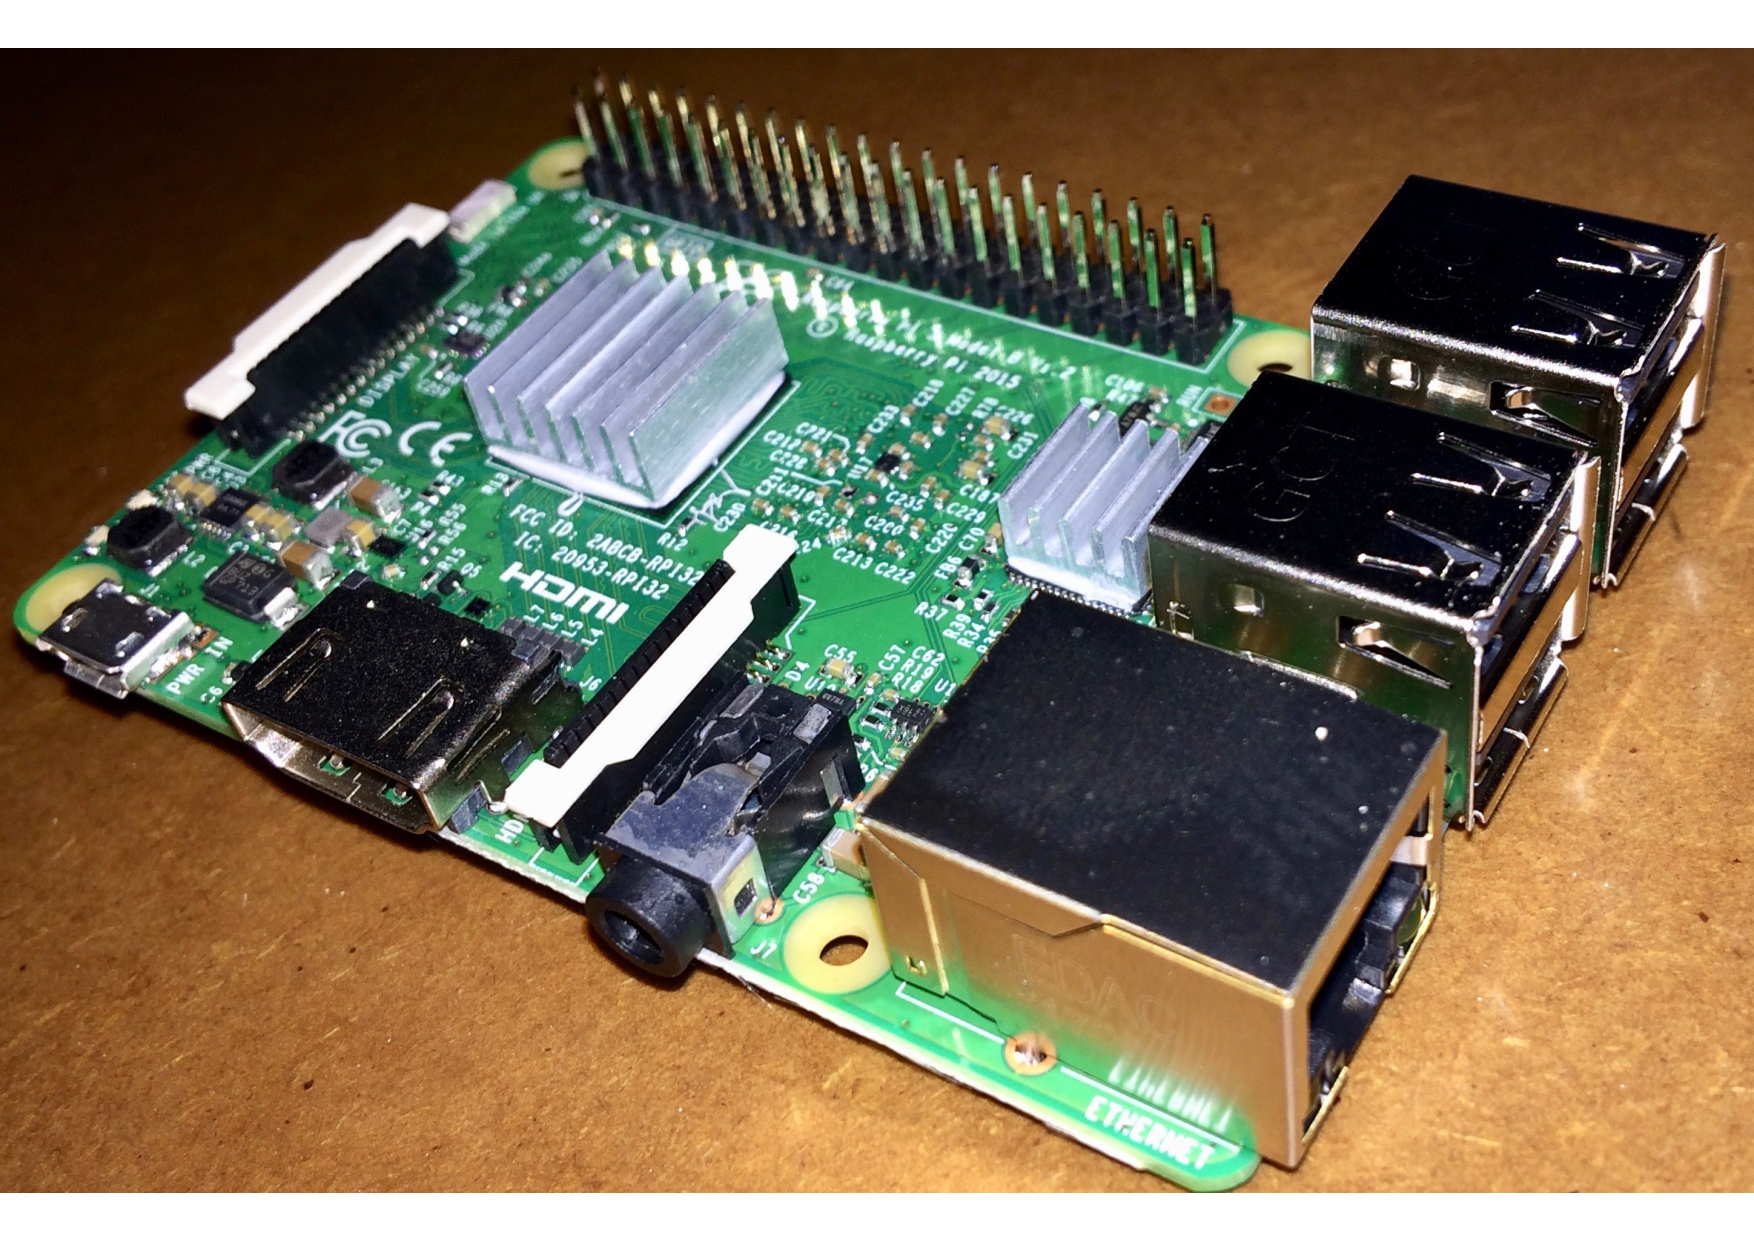
\includegraphics[width=0.9\textwidth]{raspi}
	\caption{Raspberry Pi 3.}\label{fig:raspi3b}
\end{figure}

Una vez descargado el sistema, este ha sido instalado en una micro SD mediante el siguiente procedimiento por consola\footnote{Realizado en OSX, aunque en Linux es muy similar}:
\begin{itemize}
\item\code{diskutil list} Permite localizar el dispositivo en el que se encuentra la tarjeta. En nuestro caso \code{/dev/disk4}
\item\code{diskutil umountDisk /dev/disk4} Permite desmontar el volumen. 
\item\code{sudo dd if=raspbian-stretch.img of=/dev/rdisk4 bs=1m} El comando \code{dd} copia la entrada estándar a la salida estándar. Mediante \code{if/of} se establece el fichero de entrada/salida. Mediante \code{bs} se establece el tamaño de bloque a copiar. Se está utilizando \code{/dev/\underline{\textbf{r}}disk4} en lugar de \code{/dev/disk4} debido a la capacidad de OSX de trabajar con dispositivos en bruto, \textit{raw}, de forma que es posible acceder al dispositivo de forma directa\footnote{Véase \code{man hdiutil}, sección \textit{DEVICE SPECIAL FILES}}, sin almacenar en un buffer la lectura del archivo, proporcionando velocidades de escritura/lectura hasta 20 veces más rápidas.
\end{itemize}


Una vez realizados estos pasos, se puede insertar la microSD en la Raspberry Pi. Para encenderla basta con utilizar el puerto micro-usb de que dispone.\\La Raspberry Pi 3 requiere de una fuente de alimentación capaz de proporcionar 2,5A\footnote{Véase https://www.raspberrypi.org/help/faqs/\#power} para funcionar al máximo nivel de estrés para el procesador y alimentar dispositivos USB.

Sin embargo, este no es estrictamente nuestro caso, véase el apartado \hyperref[subsec:Modificaciones]{Modificaciones}. Se requiere un dispositivo cuyo consumo sea lo más reducido posible, pero que sea rápido en la ejecución, y que muestre poca latencia en operaciones de \code{IO}, que es donde se encuentra el cuello de botella.

Una vez encendida, se accede a ella con el usuario por defecto \code{pi} y la contraseña por defecto \code{raspberry}. Obviamente ambas \textbf{han sido cambiadas} por motivos de seguridad.



\subsubsection{Modificaciones}
\label{subsec:Modificaciones}

\begin{figure}
	\centering
	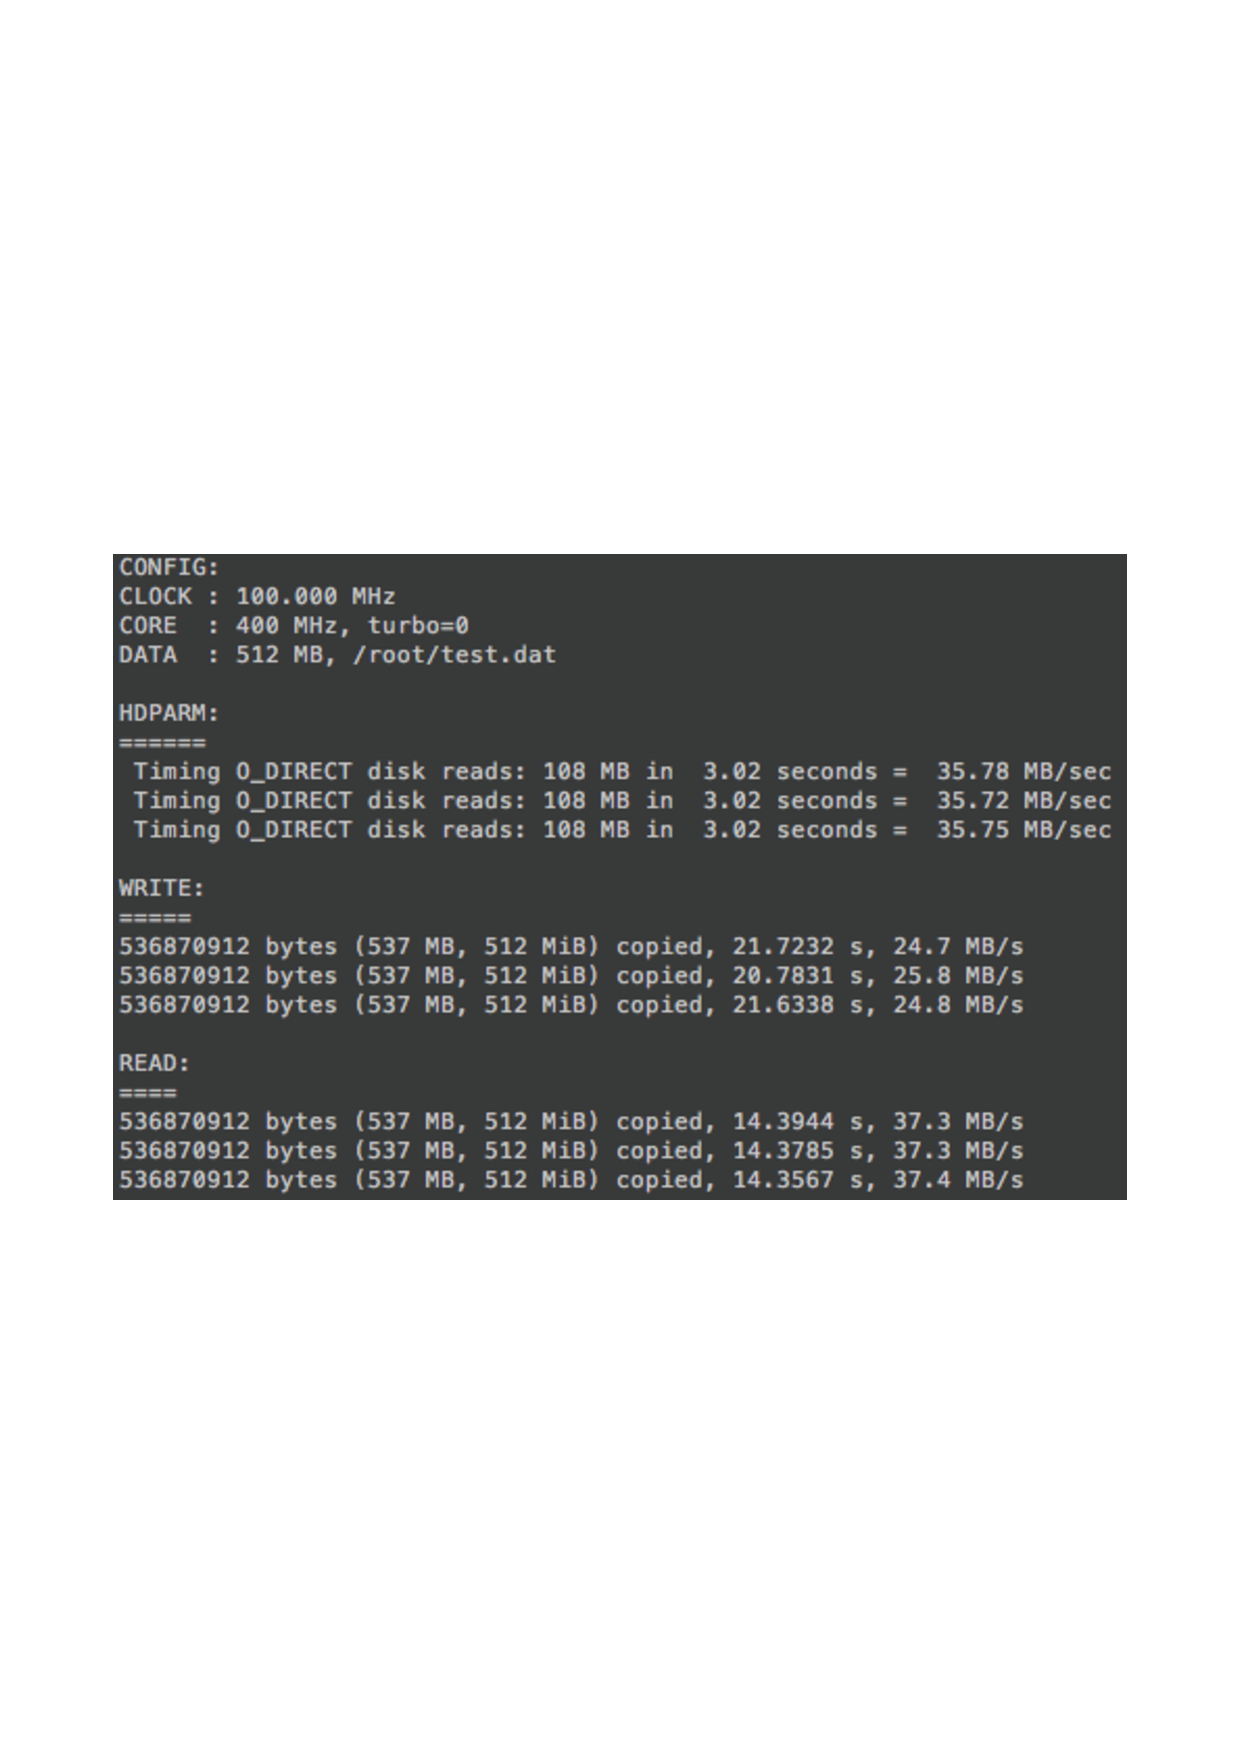
\includegraphics[width=0.9\textwidth]{sdbench}
	\caption{Benchmark de lector microSD OC.}\label{fig:sdbenchmark}
\end{figure}

\begin{itemize}
\item Se ha desactivado el puerto HDMI para reducir el consumo en \textasciitilde{}30mA: \\Para ello se ha incluido en \code{/etc/rc.local} la línea \code{/usr/bin/tvservice -o}.
\item Se ha overclockeado el lector de microSD a 100MHz, en lugar de los 50MHz por defecto: \\Para ello se ha incluido en \code{/boot/config.txt} la línea \code{dtparam=sd\_overclock=100}.\\Y que arroja los resultados mostrados en la imagen \ref{fig:sdbenchmark}
\item Se han incluido una serie de disipadores para evitar sobrecalentamiento de la placa. Así como un pequeño ventilador de bajo consumo.
\end{itemize} 


\subsection{Controladora de Vuelo}

Una controladora de vuelo (\textit{FC} de aquí en adelante) es un pequeño circuito integrado, que contiene un procesador, una serie de sensores, y una serie de entradas y salidas. 
\begin{figure}
\centering
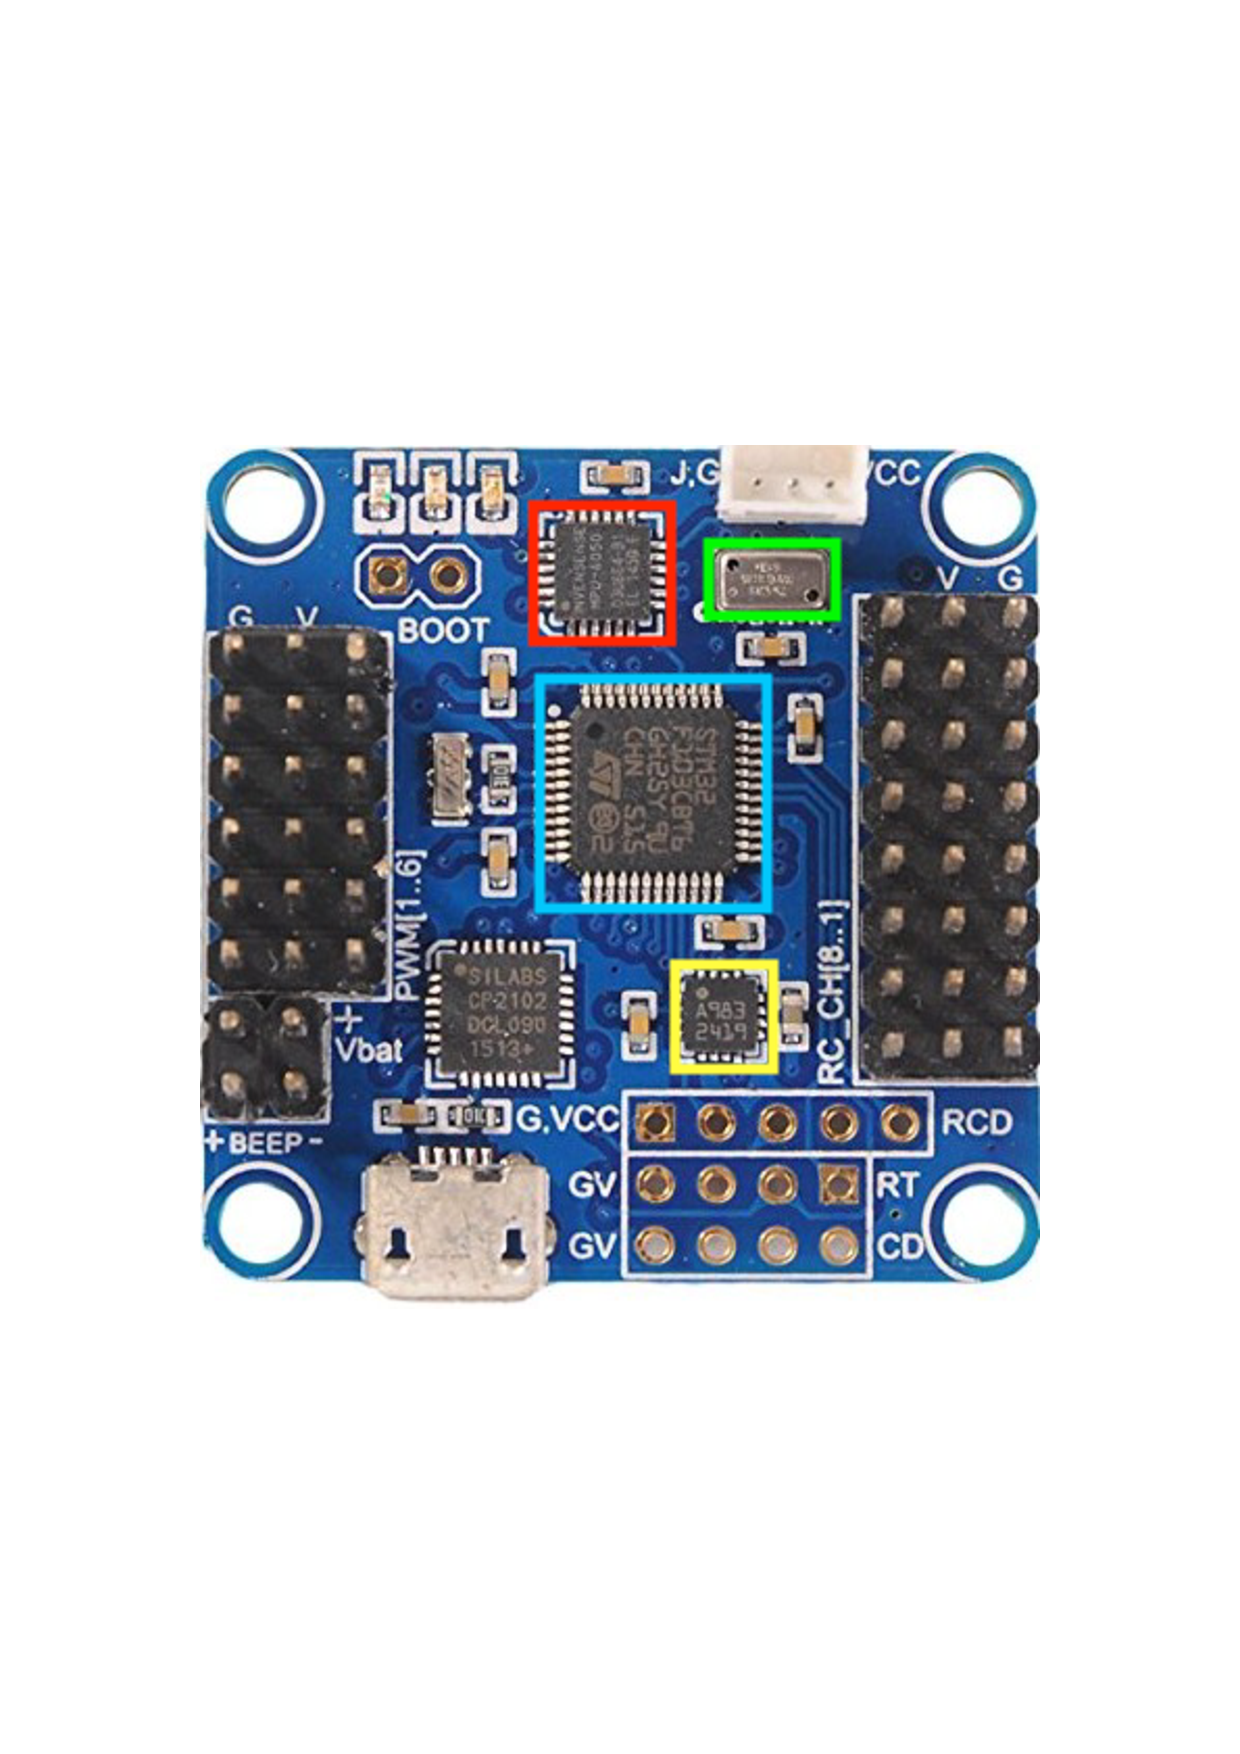
\includegraphics[width=0.5\textwidth]{flip32}
\caption{Controladora de Vuelo Flip32.}\label{fig:fc}
\end{figure}
La FC se encarga de mantener el sistema de estabilización del drone, tomando medidas de los sensores de que dispone, tales como un acelerómetro, giroscopio, magnetómetro, barómetro... etc. 

En el caso de la FC usada para este proyecto, llamada Flip32 y mostrada en la imagen \ref{fig:fc}, se dispone de un IC MPU-6050, en rojo, con acelerómetro y giroscopio, así como de un barómetro M55611, en verde, y un magnetómetro HMC5883L, en amarillo.
El núcleo de esta pequeña placa es un procesador STM32F103, en cyan, a 72MHz y basado en arquitectura ARM el cual dispone de dos puertos serie, que permiten establecer comunicación entre la FC y otros dispositivos, como emisoras u otros sensores.

El puerto micro-USB de que dispone es utilizado para establecer comunicación entre el configurador de opciones del drone, o en el caso de nuestro proyecto, para hacer uso del \hyperref[subsec:MSP]{MultiWii Serial Protocol}. 


\subsubsection{Entradas}
En el lado derecho de la imagen \ref{fig:fc} pueden verse una serie de pines que actúan como 8 canales de entrada desde el receptor de radio.
Dichos canales de entrada, por defecto, reciben una señal modulada en ancho de pulso o \hyperref[subsec:PWM]{PWM}

 

\subsubsection{Salidas}
En el lado izquierdo de la imagen \ref{fig:fc}, pueden verse otros pines que actúan como salida de señal hacia los controladores de velocidad de los motores del drone (ESC o \textit{Electronic Speed Controller}).
Estos pines de salida, emiten una señal que será interpretada por los ESC del drone, para determinar la frecuencia dada al voltaje que alimenta los motores. En el caso de nuestro proyecto, los ESC disponibles reciben una señal PWM, al igual que la FC desde un receptor de radio.

\newpage
\subsubsection{Sensores}
La controladora de vuelo Flip32 en su versión más completa, dispone de los siguientes sensores:
\begin{itemize}
\item IMU\footnote{Unidad de Medición Inercial.} MPU-6050: Se trata de un circuito integrado compuesto de un acelerómetro de tres (3) ejes y un giroscopio de tres (3) ejes. El acelerómetro mide las fuerzas en los tres diferentes ejes (en \textit{g}) , el giroscopio se encarga de medir la velocidad angular en cada uno de los tres ejes (en degº/s )
\item Magnetómetro HMC5883L: Se trata de un pequeño magnetómetro digital capaz de medir el campo magnético terrestre (en Gauss). Se debe tener en cuenta que según la posición en el planeta, el campo magnético varía entre \si{\gauss{0.25}} - \si{\gauss{0.65}}, así como la declinación magnética de la zona en la que se realiza la medición.\footnote{Disponible en: http://magnetic-declination.com/}
\item Barómetro M55611: Se trata de un altímetro de alta precisión, con resoluciones de hasta 10cm, que funciona midiendo la presión atmosférica (en milibar). Hay que tener en cuenta que los cambios de presión, como los generados por las hélices del drone, hace variar la medida del sensor. Por ello, en el caso de usarlo, se cubre con un pequeño filtro de un material absorbente.
\end{itemize}
\newpage
\section{Protocolos}

\subsection{Pulse Width Modulation}
\label{subsec:PWM}

\externaldocument[5-]{./tex/5_Aspectos_relevantes_del_desarrollo_del_proyecto}

La modulación por ancho de pulso, se basa en medir el transcurso de tiempo entre el flanco de subida de una señal, y el flanco de bajada, tal y como puede verse en la imágen \ref{fig:PWM}.
En este contexto, un receptor de radio recibe una señal de la emisora,  y genera una señal PWM acorde que será transmitida a la FC.
Estas son capaces de entender señales de entre 1000 y 2000\si{\us}. Cualquier valor por debajo, o por encima, haría entrar la controladora en FailSafe\footnote{Al recibir una señal inválida por parte del receptor, la controladora de vuelo puede ser configurada para desactivar el drone, mantener la última medida buena conocida, intentar aterrizar... etc. Este modo es conocido como FailSafe}
En el caso de este proyecto, se ha determinado que no se hará uso de este protocolo para la comunicación entre la Raspberry Pi y la controladora de vuelo, véase \ref{5-sec:MSP_implementation} y \ref{subsec:MSP}, y por lo tanto el uso de estos pines queda descartado.

Sin embargo, la comunicación entre la FC y los ESC se realiza mediante este tipo de señal, por ello se ha considerado relevante explicar, brevemente, su funcionamiento.
\begin{figure}
	\centering
	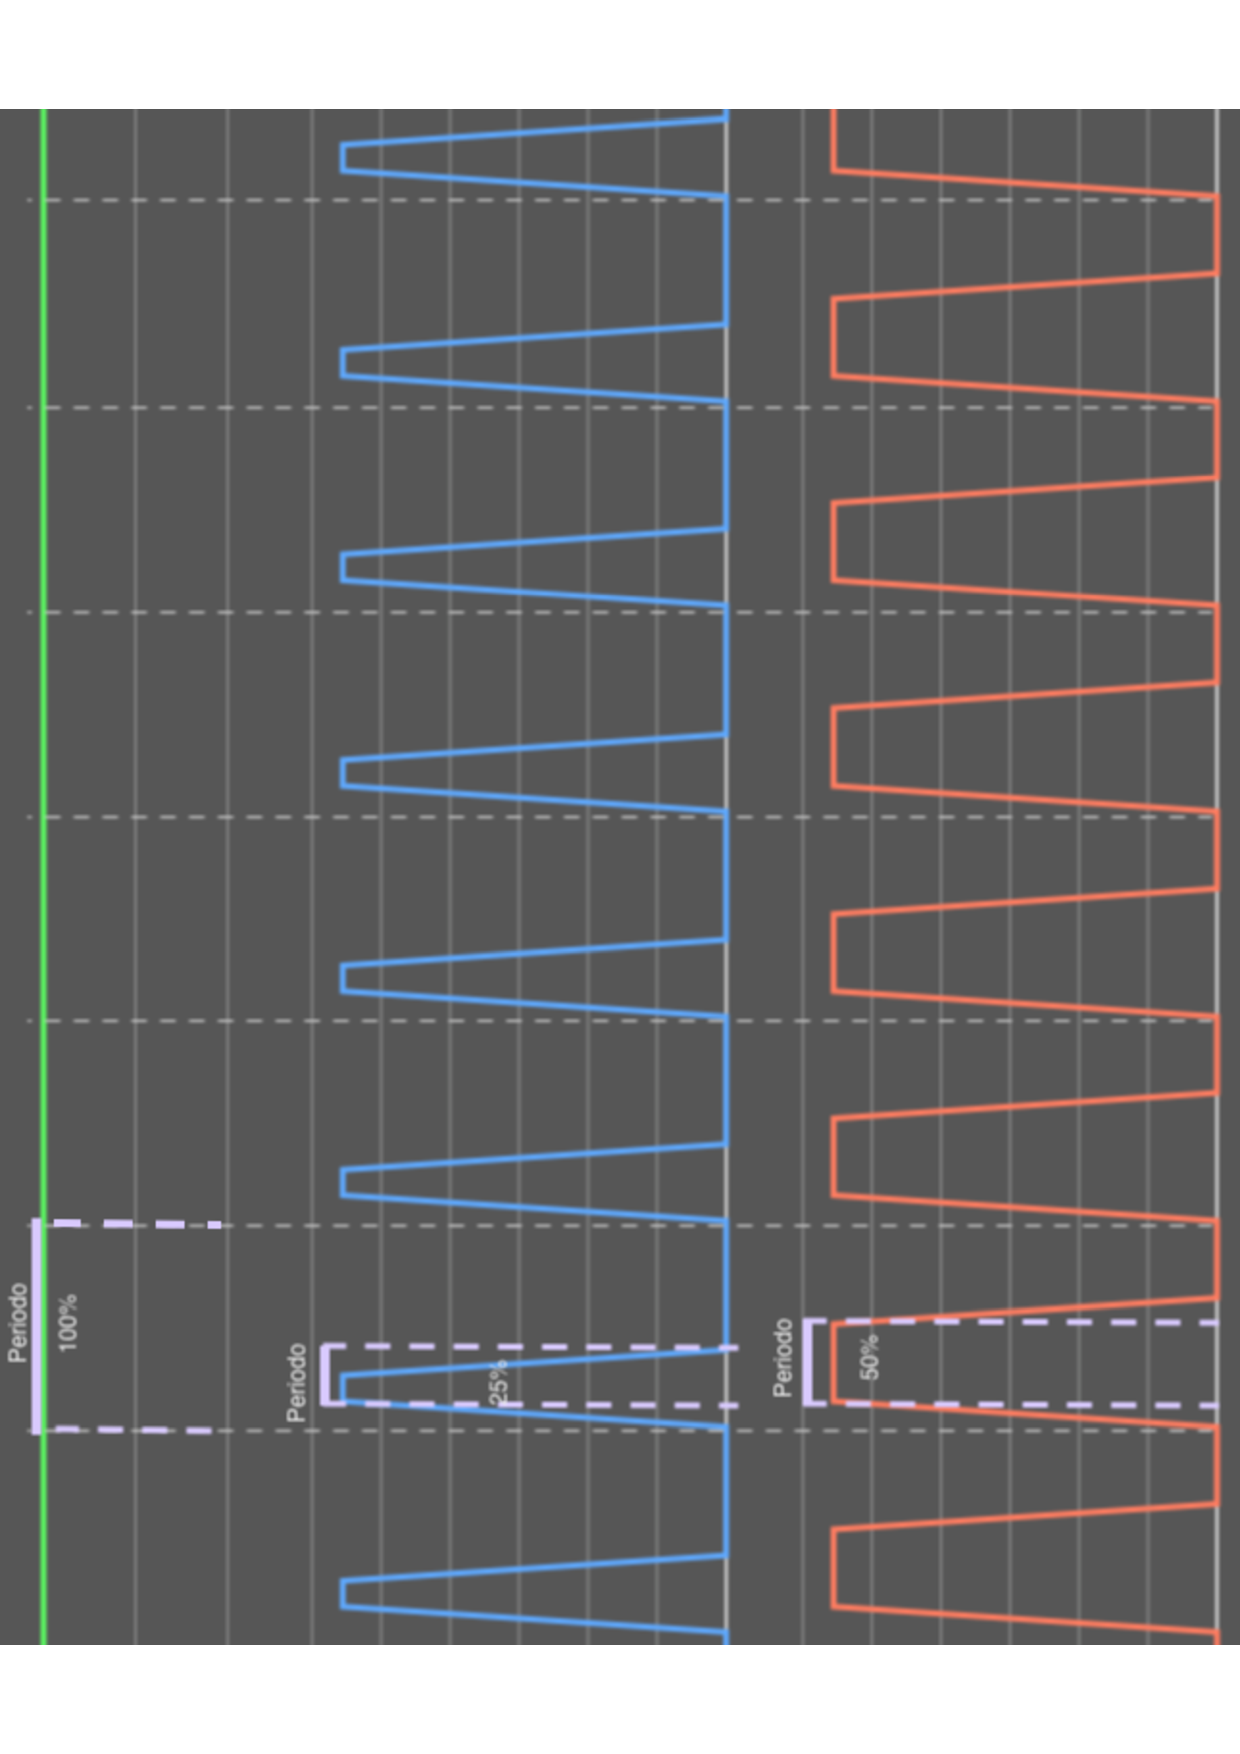
\includegraphics[width=0.9\textwidth]{PWM}
	\caption{Modulación en Ancho de Pulso. Arriba 100\% del ciclo usado. Centro 25\% del ciclo usado. Abajo 50\% del ciclo usado}\label{fig:PWM}
\end{figure}


\subsection{MultiWii Serial Protocol}
\label{subsec:MSP}

MultiWii es un software de control de multirotores y está basado en componentes de la Nintendo Wii. Los mandos de control de la consola de Nintendo poseen tres acelerómetros para determinar la posición angular y medir aceleraciones laterales. El problema es que los acelerómetros no son precisos para variaciones pequeñas, de forma que Nintendo creó un complemento que se podía conectar al propio mando, el Wii Motion Plus, que dispone de tres giroscopios, de forma que unidos a los tres acelerómetros iniciales, proporcionan una medición mucho más precisa de la posición del mando.

Para crear un entorno amigable para el usuario común, se desarrolló una aplicación de escritorio capaz de configurar los parámetros de esta controladora de vuelo poco convencional. De alguna forma debía lograrse una comunicación entre la FC y la aplicación, y así se implementó MultiWii Serial Protocol.\\Conocido como \textit{MSP}, se trata de un protocolo que se ha mantenido en diferentes implementaciones de sistemas de control de vuelo. No solo aquellos basados en sensores de la Nintendo Wii controlados por Arduino, sino en otros más modernos y potentes que han ido surgiendo los últimos años. Como el utilizado en nuestro proyecto.

Se trata de un protocolo eficiente y sencillo, que permite una comunicación rápida y completa. Su composición puede verse en la imagen \ref{fig:MSPlayout}
\begin{figure}
	\centering
	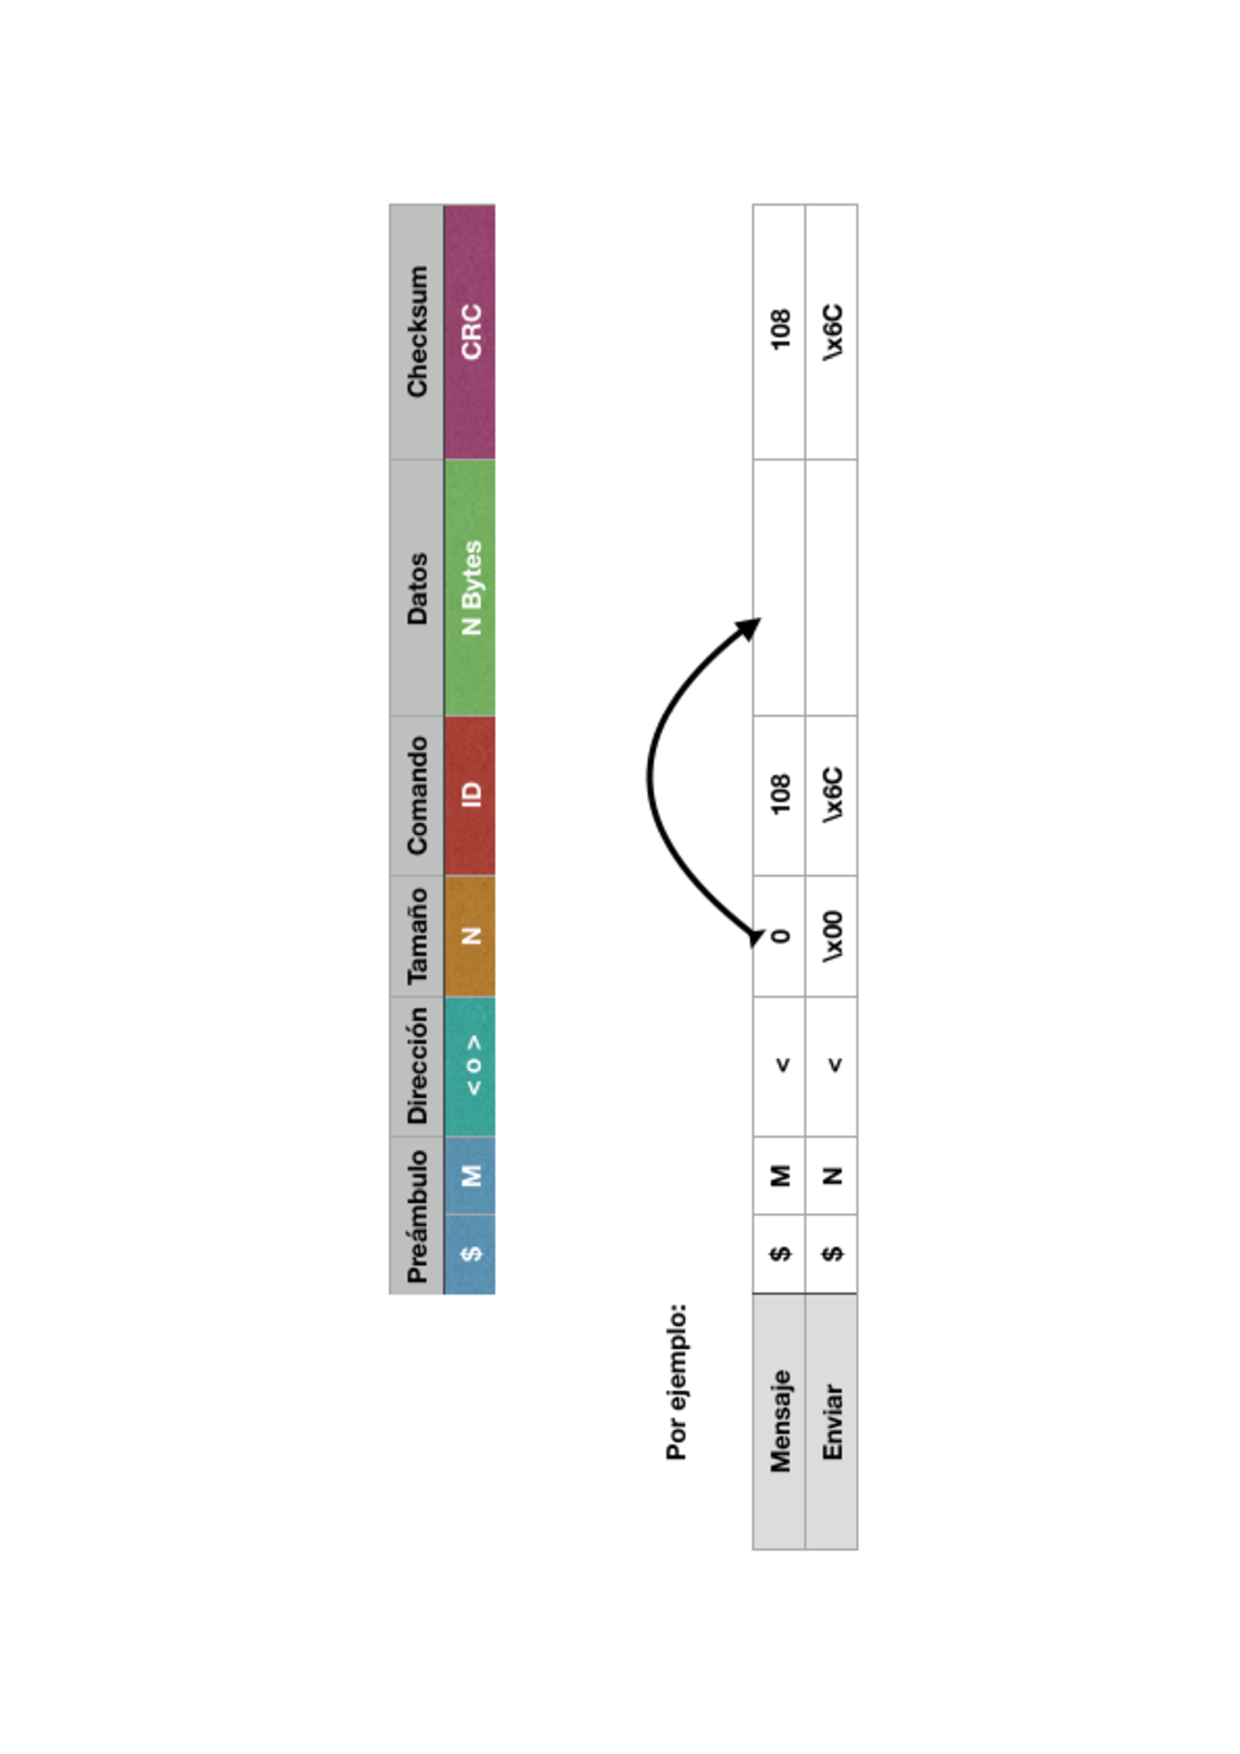
\includegraphics[width=0.9\textwidth]{MSPlayout}
	\caption{Composición de un mensaje MSP}\label{fig:MSPlayout}
\end{figure}

\begin{itemize}
\item Preámbulo: Se trata de dos caracteres ASCII que determinan el comienzo de un nuevo mensaje. Se compone de un símbolo '\$' y una letra 'M'.
\item Dirección: Se trata de un caracter ASCII que determina la dirección del mensaje, \textbf{hacia} la controladora '<' o \textbf{desde} la controladora '>'.
\item Tamaño: Se trata de un byte que determina el tamaño, en bytes, de los datos enviados o recibidos.
\item Comando: Se trata de un byte que determina el comando a ejecutar. Véase \ref{5-sec:MSP_implementation} para una relación de los comandos implementados.
\item Datos: Se trata de una serie de bytes, de longitud definida por el byte <\textit{tamaño}>, que establecen el resto de parámetros a pasar con la función definida por el byte <\textit{comando}>.
\item Checksum: Se trata de un byte de control. Se define su valor mediante la función XOR entre <\textit{tamaño}>, <\textit{comando}> y cada byte contenido en <\textit{datos}>


\end{itemize}

En el caso de nuestro proyecto, se hará uso de este protocolo dado que existe la posibilidad de establecer la recepción de los canales de radio a través de un puerto serie. Es decir, en lugar de utilizar un receptor de radio, se utilizará un puerto serie para obtener la telemetría\footnote{Se define telemetría como un sistema de medición de magnitudes a distancia; en este contexto el término se ha desvirtuado y se entiende como la información que es transmitida de vuelta a la emisora de vuelo, siendo esta generalmente información de los sensores de la FC, GPS o voltaje disponible en la batería.}, y establecer las entradas de los canales de radio.






\section{Referencias}

Las referencias se incluyen en el texto usando cite \cite{wiki:latex}. Para citar webs, artículos o libros \cite{koza92}.


\section{Imágenes}

Se pueden incluir imágenes con los comandos standard de \LaTeX, pero esta plantilla dispone de comandos propios como por ejemplo el siguiente:

\imagen{escudoInfor}{Autómata para una expresión vacía}



\section{Listas de items}

Existen tres posibilidades:

\begin{itemize}
	\item primer item.
	\item segundo item.
\end{itemize}

\begin{enumerate}
	\item primer item.
	\item segundo item.
\end{enumerate}

\begin{description}
	\item[Primer item] más información sobre el primer item.
	\item[Segundo item] más información sobre el segundo item.
\end{description}
	
\begin{itemize}
\item 
\end{itemize}

\section{Tablas}

Igualmente se pueden usar los comandos específicos de \LaTeX o bien usar alguno de los comandos de la plantilla.

\tablaSmall{Herramientas y tecnologías utilizadas en cada parte del proyecto}{l c c c c}{herramientasportipodeuso}
{ \multicolumn{1}{l}{Herramientas} & App AngularJS & API REST & BD & Memoria \\}{ 
HTML5 & X & & &\\
CSS3 & X & & &\\
BOOTSTRAP & X & & &\\
JavaScript & X & & &\\
AngularJS & X & & &\\
Bower & X & & &\\
PHP & & X & &\\
Karma + Jasmine & X & & &\\
Slim framework & & X & &\\
Idiorm & & X & &\\
Composer & & X & &\\
JSON & X & X & &\\
PhpStorm & X & X & &\\
MySQL & & & X &\\
PhpMyAdmin & & & X &\\
Git + BitBucket & X & X & X & X\\
Mik\TeX{} & & & & X\\
\TeX{}Maker & & & & X\\
Astah & & & & X\\
Balsamiq Mockups & X & & &\\
VersionOne & X & X & X & X\\
} 

\capitulo{4}{Técnicas y herramientas}

Esta parte de la memoria tiene como objetivo presentar las técnicas metodológicas y las herramientas de desarrollo que se han utilizado para llevar a cabo el proyecto. Si se han estudiado diferentes alternativas de metodologías, herramientas, bibliotecas se puede hacer un resumen de los aspectos más destacados de cada alternativa, incluyendo comparativas entre las distintas opciones y una justificación de las elecciones realizadas. 
No se pretende que este apartado se convierta en un capítulo de un libro dedicado a cada una de las alternativas, sino comentar los aspectos más destacados de cada opción, con un repaso somero a los fundamentos esenciales y referencias bibliográficas para que el lector pueda ampliar su conocimiento sobre el tema.



\capitulo{5}{Aspectos relevantes del desarrollo del proyecto}

Este apartado pretende recoger los aspectos más interesantes del desarrollo del proyecto, comentados por los autores del mismo.
Debe incluir desde la exposición del ciclo de vida utilizado, hasta los detalles de mayor relevancia de las fases de análisis, diseño e implementación.
Se busca que no sea una mera operación de copiar y pegar diagramas y extractos del código fuente, sino que realmente se justifiquen los caminos de solución que se han tomado, especialmente aquellos que no sean triviales.
Puede ser el lugar más adecuado para documentar los aspectos más interesantes del diseño y de la implementación, con un mayor hincapié en aspectos tales como el tipo de arquitectura elegido, los índices de las tablas de la base de datos, normalización y desnormalización, distribución en ficheros3, reglas de negocio dentro de las bases de datos (EDVHV GH GDWRV DFWLYDV), aspectos de desarrollo relacionados con el WWW...
Este apartado, debe convertirse en el resumen de la experiencia práctica del proyecto, y por sí mismo justifica que la memoria se convierta en un documento útil, fuente de referencia para los autores, los tutores y futuros alumnos.

\capitulo{6}{Trabajos relacionados}

Este apartado sería parecido a un estado del arte de una tesis o tesina. En un trabajo final grado no parece obligada su presencia, aunque se puede dejar a juicio del tutor el incluir un pequeño resumen comentado de los trabajos y proyectos ya realizados en el campo del proyecto en curso. 

\capitulo{7}{Conclusiones y Líneas de trabajo futuras}

Todo proyecto debe incluir las conclusiones que se derivan de su desarrollo. Éstas pueden ser de diferente índole, dependiendo de la tipología del proyecto, pero normalmente van a estar presentes un conjunto de conclusiones relacionadas con los resultados del proyecto y un conjunto de conclusiones técnicas. 
Además, resulta muy útil realizar un informe crítico indicando cómo se puede mejorar el proyecto, o cómo se puede continuar trabajando en la línea del proyecto realizado. 



\bibliographystyle{plain}
\bibliography{bibliografia}

\end{document}
